% This file was created with tikzplotlib v0.10.1.
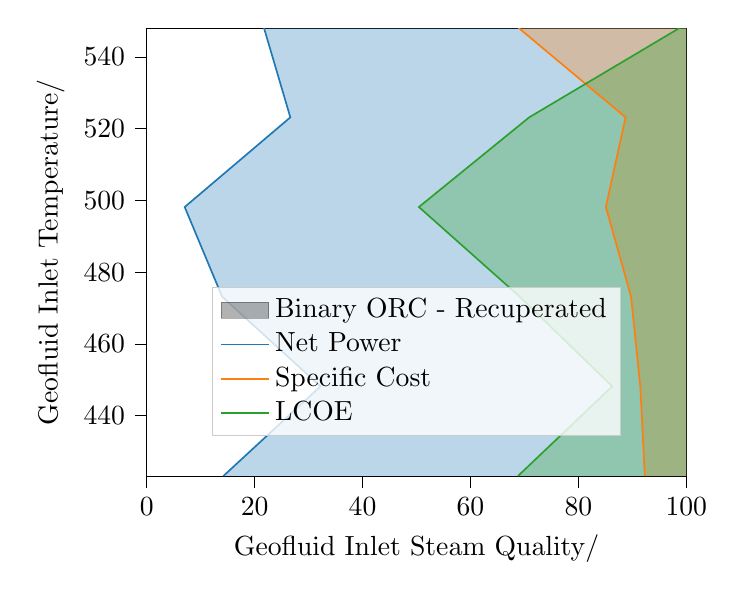
\begin{tikzpicture}

\definecolor{darkgray176}{RGB}{176,176,176}
\definecolor{darkorange25512714}{RGB}{255,127,14}
\definecolor{forestgreen4416044}{RGB}{44,160,44}
\definecolor{lightgray204}{RGB}{204,204,204}
\definecolor{steelblue31119180}{RGB}{31,119,180}

\begin{axis}[
legend cell align={left},
legend style={
  fill opacity=0.8,
  draw opacity=1,
  text opacity=1,
  at={(0.5,0.09)},
  anchor=south,
  draw=lightgray204
},
tick align=outside,
tick pos=left,
x grid style={darkgray176},
xlabel={Geofluid Inlet Steam Quality/\unit{\percent}},
xmin=0, xmax=100,
xtick style={color=black},
y grid style={darkgray176},
ylabel={Geofluid Inlet Temperature/\unit{\K}},
ymin=423, ymax=548,
ytick style={color=black}
]
\path [draw=black, fill=black, opacity=0.3]
(axis cs:0,551)
--(axis cs:0,550)
--(axis cs:100,550)
--(axis cs:100,551)
--(axis cs:100,551)
--(axis cs:0,551)
--cycle;
\addlegendimage{area legend, draw=black, fill=black, opacity=0.3}
\addlegendentry{Binary ORC 
- Recuperated}

\path [fill=steelblue31119180, fill opacity=0.3]
(axis cs:100,548.15)
--(axis cs:21.7242033806414,548.15)
--(axis cs:26.6217678807088,523.15)
--(axis cs:7.04779422979273,498.15)
--(axis cs:13.9829173855952,473.15)
--(axis cs:32.2017990765065,448.15)
--(axis cs:14.2137514980781,423.15)
--(axis cs:100,423.15)
--(axis cs:100,423.15)
--(axis cs:100,448.15)
--(axis cs:100,473.15)
--(axis cs:100,498.15)
--(axis cs:100,523.15)
--(axis cs:100,548.15)
--cycle;

\path [fill=darkorange25512714, fill opacity=0.3]
(axis cs:100,423.15)
--(axis cs:92.3043476893073,423.15)
--(axis cs:91.4697004448753,448.15)
--(axis cs:89.7592524624038,473.15)
--(axis cs:85.0890435171186,498.15)
--(axis cs:88.7420889520287,523.15)
--(axis cs:68.8712138091157,548.15)
--(axis cs:100,548.15)
--(axis cs:100,548.15)
--(axis cs:100,523.15)
--(axis cs:100,498.15)
--(axis cs:100,473.15)
--(axis cs:100,448.15)
--(axis cs:100,423.15)
--cycle;

\path [fill=forestgreen4416044, fill opacity=0.3]
(axis cs:100,548.15)
--(axis cs:98.841651060356,548.15)
--(axis cs:70.8815732826621,523.15)
--(axis cs:50.4467089009602,498.15)
--(axis cs:69.123214997554,473.15)
--(axis cs:86.27857725011,448.15)
--(axis cs:68.8069805799256,423.15)
--(axis cs:100,423.15)
--(axis cs:100,423.15)
--(axis cs:100,448.15)
--(axis cs:100,473.15)
--(axis cs:100,498.15)
--(axis cs:100,523.15)
--(axis cs:100,548.15)
--cycle;

\addplot [semithick, steelblue31119180]
table {%
21.7242033806414 548.15
26.6217678807088 523.15
7.04779422979273 498.15
13.9829173855952 473.15
32.2017990765065 448.15
14.2137514980781 423.15
};
\addlegendentry{Net Power}
\addplot [semithick, darkorange25512714]
table {%
92.3043476893073 423.15
91.4697004448753 448.15
89.7592524624038 473.15
85.0890435171186 498.15
88.7420889520287 523.15
68.8712138091157 548.15
};
\addlegendentry{Specific Cost}
\addplot [semithick, forestgreen4416044]
table {%
98.841651060356 548.15
70.8815732826621 523.15
50.4467089009602 498.15
69.123214997554 473.15
86.27857725011 448.15
68.8069805799256 423.15
};
\addlegendentry{LCOE}
\end{axis}

\end{tikzpicture}
